\chapter{Results}
\label{results}
The \Cref{sec-cloud} transition to a renewed cloud-based architecture enhances performance, scalability, and reliability. \Cref{sub-comunication} covers communication improvements with more efficient architecture, while \Cref{sub-storage} discusses storage and database enhancements to increase speed and reliability. The \Cref{sec-packages} explains the package architecture improvement for the tool. The \Cref{sec-services-behaivour} explains the improvements in the tool and its features. In \Cref{sec-tests-2.0} shows how the tool interface works. The \Cref{sub-testing-article} explains how the tool was tested with the projects given by the articles. The \Cref{sub-testing-real} explains how the tool was tested with real-world projects.
The \Cref{sec-comparing} explains the comparison between the tool versions. The \Cref{sec-closing-results} have remarks for the section.


\textcolor{red}{lembrar de fazer o preâmbulo como fez para os outros capítulos
1 - RMT 2.0\\
2 - Testes com projetos\\
3 - Comparação da RMT 1 com 2
}

\section{The Renewed Cloud Based Architecture}
\label{sec-cloud}
The revised architecture introduces modifications to the communication protocols between services. The initial version of the tool had three services and one Java desktop application. The revised architecture transitioned the desktop application to a web-based platform, altering each service's operational dynamics. The newly devised architecture is illustrated in \Cref{fig-async}.

The system architecture contains three distinct microservices dedicated to process management, supported by two communication queues and partitioned storage solutions having two distinct buckets: one designated for original projects and the other for refactored projects. The database infrastructure leverages an ElastiCache, while a load balancer is utilized to efficiently distribute incoming requests originating from the gateway.


\textcolor{red}{o numero da figura está errado. A última foi 17 e agora deveria ser 18. Deveria comentar um pouco sobre a figura em alto nível antes de entrar nas seções. Cada seção vai falar de um item que melhorou. Deve introduzir isso por meio de um texto. Para quem está lendo, isso facilita.}

\begin{figure}[ht!]
\SetCaptionWidth{\textwidth}
\caption{RMT revised architecture diagram}
\label{fig-async}
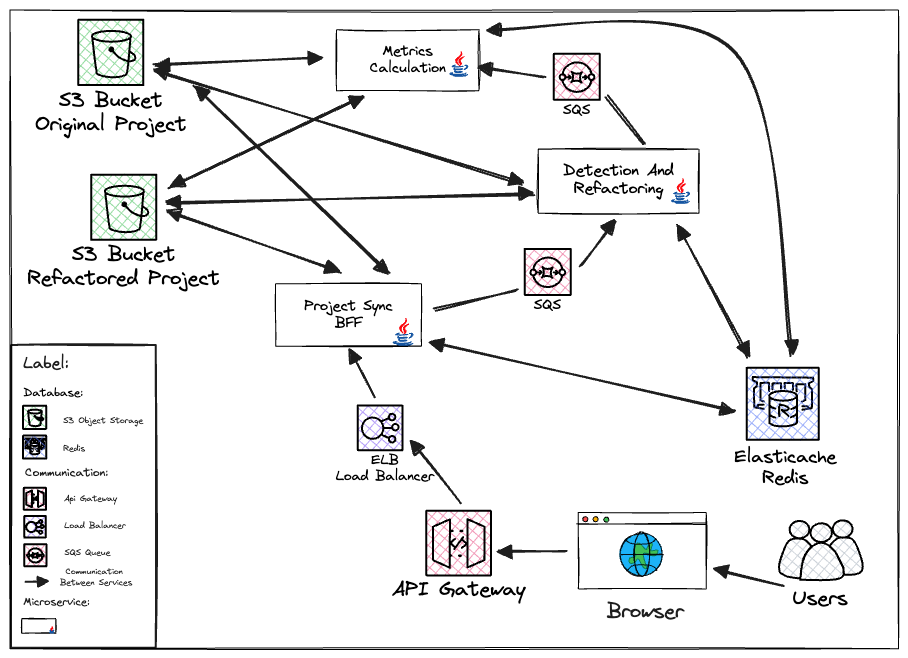
\includegraphics[width =\textwidth, scale=0.2]{Chapter-5/Figures/Async.png}
\SourceOrNote{Own authorship (2024)}
\end{figure}
\FloatBarrier

\subsection{Comunication Improvements}
\label{sub-comunication}

The communication type was switched to queues instead of HTTP requests. The modification primarily aims to establish a communication mechanism with enhanced configurability in the event of failures, as the services must acknowledge the messages, or they will be retried as often as configured. Queues also offer an asynchronous communication that is out of the box. Otherwise, in the HTTP request, the retry has to be implemented on the client side according to the server response. It is also possible to have an HTTP asynchronous request, but it must be implemented on the client side.

The Simple Queue Service (SQS) operates in its default configuration, implementing a quintuple retry mechanism to transmit a JSON object containing the project identifier between microservices.

\subsection{Storage \& Database Improvements}
\label{sub-storage}

The initial version of RMT utilizes MongoDB GridFs for file storage, a feature designed to facilitate the preservation of files within the database architecture. The updated version uses Amazon S3 for project storage, using a dual-bucket strategy: one designated for the original project and the other for the refactored iterations. All microservices are granted access to the designated buckets, enabling seamless file storage and retrieval. The project information and statuses are stored in the Redis in-memory document database, and all services have access.

\section{RMT 2.0 Packages}
\label{sec-packages}

After the architectural improvements, the package structure was reorganized and simplified. The advanced capabilities of the Spring framework, with the optimization of the codebase and the ensuring of linear communication between services, facilitated the reduction in both the number and the size of packages.

The Project Sync BFF went through a consolidation, reducing its packages from seven to five, with none of the original packages retained. The \texttt{controller} package is tasked with exposing the endpoint and initiating communication with the \texttt{refactor} package. The \texttt{refactor} package contains the entire service logic; it accesses the \texttt{ repository} package for database interactions and the \texttt{gateway} package to send messages to the subsequent service. The \texttt{configuration} package has the capability to dynamically retrieve the queue's name. Its behavior is demonstrated by the diagram on \cref{fig-project-sync-package}.

\begin{figure}[ht!]
\SetCaptionWidth{\textwidth}
\caption{Project Sync BFF package diagram}
\label{fig-project-sync-package}
\fontsize{8}{10}\selectfont
\includesvg[width =\textwidth]{Chapter-5/Figures/project-sync-bff.svg}
\SourceOrNote{Own authorship (2024)}
\end{figure}
\FloatBarrier

Progressing to the Detection and Refactoring service, a reduction in the number of packages from fourteen to seven was accomplished. The service initiates the processing via the \texttt{consumer} package, which consumes messages from a queue and retrieves a project from the database using the \texttt{repository} package as it has the database communication interface. The logic for executing refactorings is located within the \texttt{refactor} package, implementing the refactoring methods in the \texttt{methods} package, and data extraction strategies located in the \texttt{dataExtraction} package. The \texttt{gateway} package has the functionality to send messages to the queue and imports the \texttt{configuration} package to dynamically retrieve the queue name. As illustrated in \cref{fig-detection-refactoring-package}, the diagram employs two colors: yellow to signify the new packages and white to indicate the packages retained from the previous version.

\begin{figure}[ht!]
\SetCaptionWidth{\textwidth}
\caption{Detection and Refactoring service package diagram}
\label{fig-detection-refactoring-package}
\includesvg[width =\textwidth]{Chapter-5/Figures/detection-and-refactoring.svg}
\SourceOrNote{Own authorship (2024)}
\end{figure}
\FloatBarrier

The Metrics Calculator has undergone a reduction from thirteen to six packages. Consistent with the behavior of the previous service, the process starts with the \texttt{consumer} package, which retrieves messages from the queue and communicates with the database via the interface provided by the \texttt{repository} package. The retrieved database results are then used to compute quality attributes within the packages \texttt{quallityAtrributes} and \texttt{calculator}, which rely on metrics generated by the \texttt{metris} packages. The \texttt{configuration} package is responsible for instantiating the CK library \textcite{ck} for the Spring framework, allowing its injection as a dependency. The corresponding diagram is illustrated in \Cref{fig-metrics-calculator-package}, highlighting the new packages in yellow and those retained from the initial version in white.

\begin{figure}[ht!]
\SetCaptionWidth{\textwidth}
\caption{Metrics Calculator service package diagram}
\label{fig-metrics-calculator-package}
\includesvg[width =\textwidth]{Chapter-5/Figures/metrics-calculator.svg}
\SourceOrNote{Own authorship (2024)}
\end{figure}
\FloatBarrier



\section{Services Behavior Improviments}
\label{sec-services-behaivour}

Notwithstanding recent updates to the tool, its resultant behavior remains unchanged. The tool now runs with a linear execution flow, obviating the need for interservice communication during project refactoring. Given the process's asynchronous nature, users must request the completion status to display the retrieved relevant information. The process is represented in \Cref{fig-activity-diagram}, with the blue nodes representing the behavior inherited from the initial version of the tool.

\begin{figure}[ht!]
\SetCaptionWidth{\textwidth}
\caption{RMT 2.0 Activity Diagram}
\label{fig-activity-diagram}
\fontsize{5.8}{8}\selectfont
\includesvg[width =\textwidth]{Chapter-5/Figures/activity-refactored-rmt.svg}
\SourceOrNote{Own authorship (2024)}
\end{figure}
\FloatBarrier

The flow starts with the user selecting the project and sending it to the API Gateway connected to the Project Sync BFF; the service sends the project ID to the refactoring queue to start the process. The Detection and Refacred Service will immediately search for the candidates to be refactored and apply the refactoring. A message with the project ID is sent to the metrics calculation queue if any candidate is found. The Metrics Calculation Service computes the quality attributes for the project and ends the processing. The Project Sync BFF service offers a pull mechanism that consults Redis looking for a final status and, if found, returns the project information and metrics. The behavior is displayed in \Cref{fig-activity-diagram}.

\section{Testing RMT 2.0}
\label{sec-tests-2.0}

In addition to architectural improvements and code refactoring, the RMT has undergone an interface transformation by migrating from a Java-based desktop application to a browser-based one. The interface now features a selection box for project updates and two buttons, 'Evaluation' for project assessment and 'Refactor' for project refactoring. These buttons remain initially disabled, pending project selection, as depicted in \Cref{fig-factory-start}.

\begin{figure}[ht!]
\SetCaptionWidth{\textwidth}
\caption{Project Selection Page}
\label{fig-factory-start}
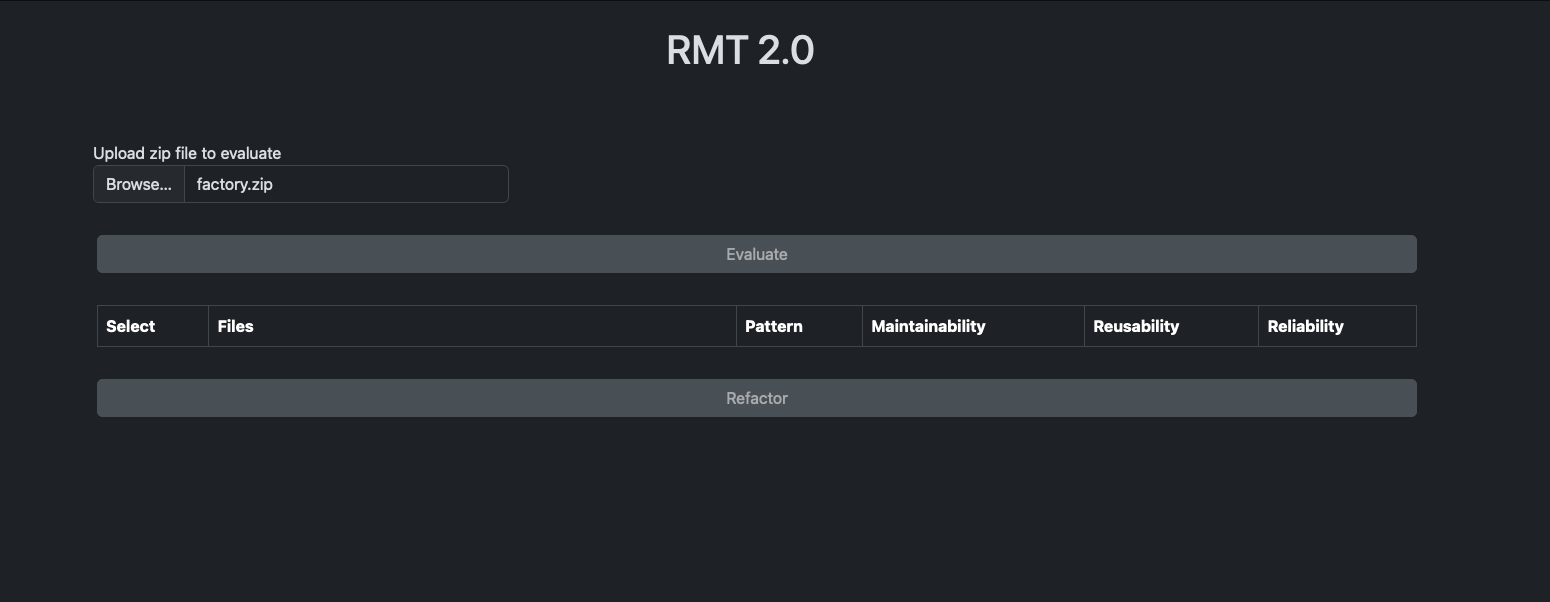
\includegraphics[width =\textwidth]{Chapter-5/Figures/rmt-factory-client-start.png}
\SourceOrNote{Own authorship (2024)}
\end{figure}
\FloatBarrier

Upon selecting the project, the 'Evaluate' button becomes active, indicated by a blue background, signifying that the project has been uploaded and the RMT backend is currently analyzing the project. This behavior is illustrated in \Cref{fig-factory-selected}.

\begin{figure}[ht!]
\SetCaptionWidth{\textwidth}
\caption{Evaluation Page}
\label{fig-factory-selected}
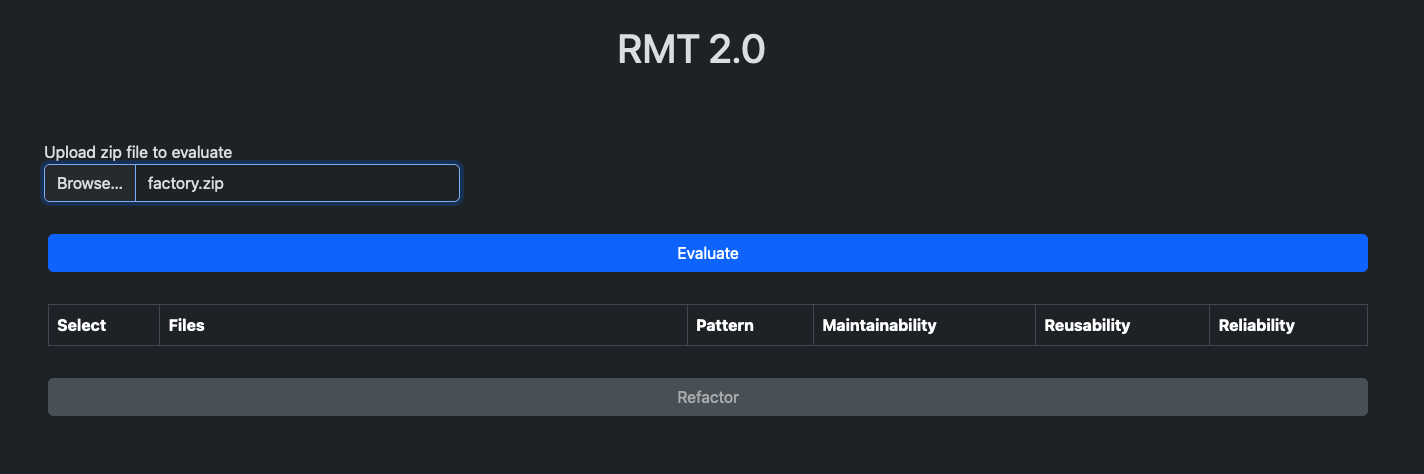
\includegraphics[width =\textwidth]{Chapter-5/Figures/rmt-factory-client-selected.png}
\SourceOrNote{Own authorship (2024)}
\end{figure}
\FloatBarrier

The refactoring candidates are shown by clicking the 'Evaluate' button. They are displayed on the table containing the refactoring information, such as the files involved, the design pattern that will be applied, and the metrics. As illustrated in \Cref{fig-factory-evaluated}.

\begin{figure}[ht!]
\SetCaptionWidth{\textwidth}
\caption{Evaluation Page}
\label{fig-factory-evaluated}
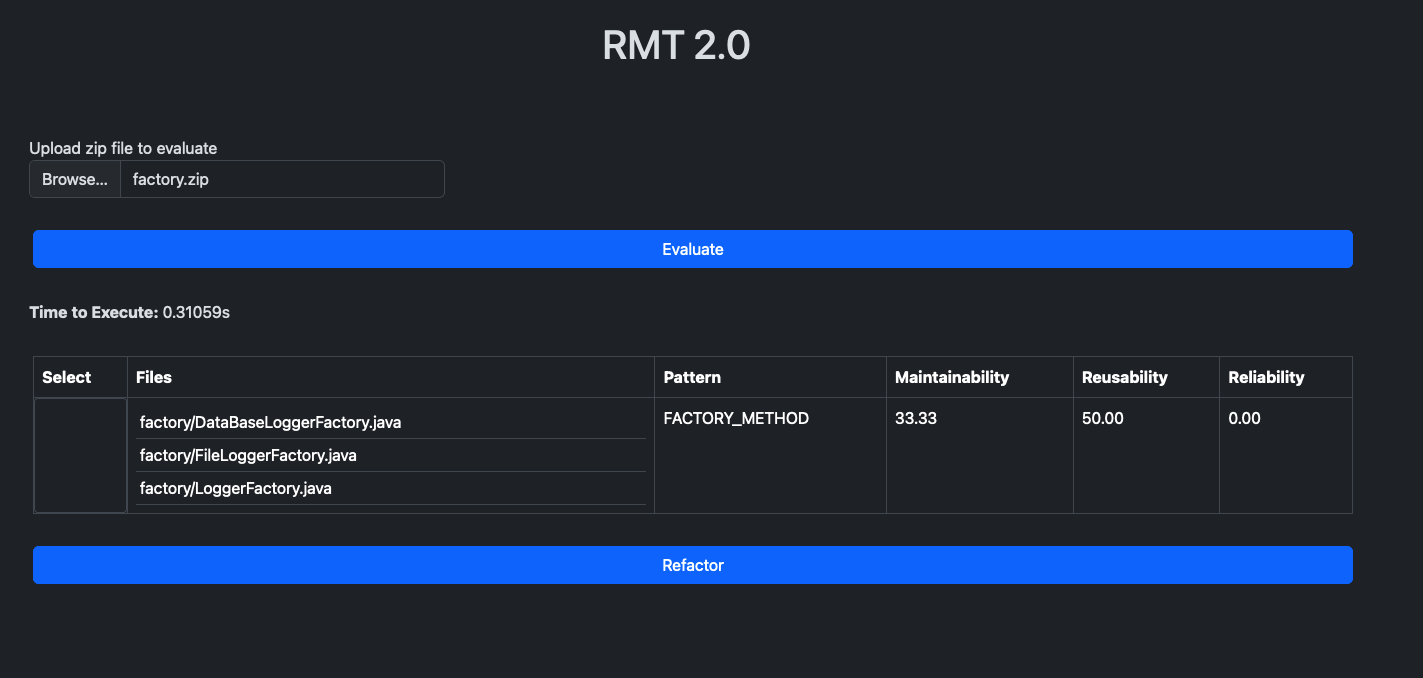
\includegraphics[width =\textwidth]{Chapter-5/Figures/rmt-factory-evaluated.png}
\SourceOrNote{Own authorship (2024)}
\end{figure}
\FloatBarrier

The refactored project can be downloaded using a link displayed after selecting a refactoring candidate in the table and clicking the 'Refactor' button. As a piece of information to the user, the elapsed time is displayed below the 'Evaluate'
 button. This is illustrated in \Cref{fig-factory-client}.

\begin{figure}[ht!]
\SetCaptionWidth{\textwidth}
\caption{Refactored Project For Factory Method Page}
\label{fig-factory-client}
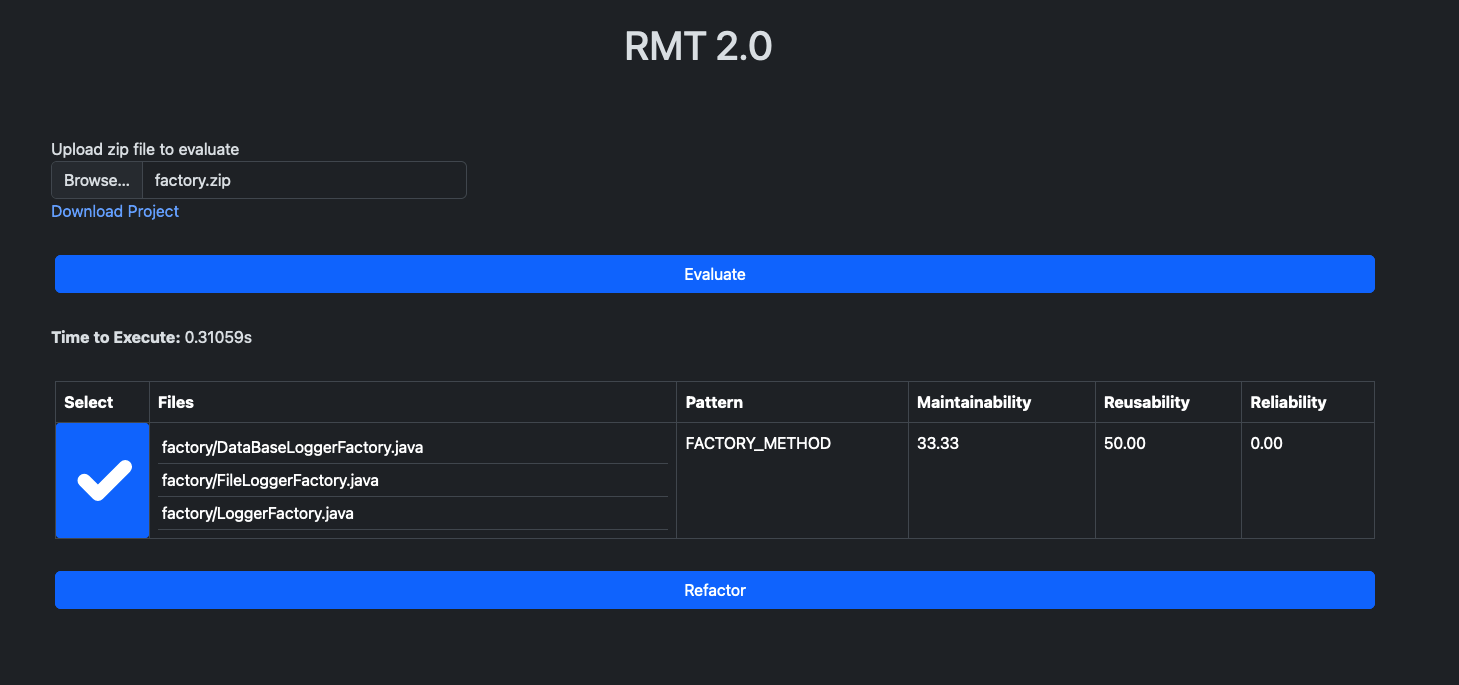
\includegraphics[width =\textwidth]{Chapter-5/Figures/rmt-factory-refactored.png}
\SourceOrNote{Own authorship (2024)}
\end{figure}
\FloatBarrier


\textcolor{red}{Pedro aqui devemos color um texto e uma image explicando o que acontece quando a pessoa aceite realizar a refatoração. Assim, fica claro o processo. O que acha?}


\subsection{Testing Through Refactored Article Application Exemplars}
\label{sub-testing-article}

The implementations exemplified by \textcite{liu2014automated} and \textcite{zafeiris2017automated} were used for the preliminary evaluation.

To refactor using the factory method design pattern, \textcite{liu2014automated} introduces four distinct classes: a \texttt{Logger} interface, 	\texttt{FileLogger} and \texttt{DatabaseLogger} which implement the interface, and the \texttt{LoggerFactory} serving as a factory to select among the implementations. The \Cref{fig-factory-client} displays the refactored \texttt{LoggerFactory} that was changed to abstract; the implementation was moved to the \texttt{FileLoggerFactory} and \texttt{DatabaseLoggerFactory}. The metrics displayed are positive, indicating an improvement in maintainability and reusability without changing reliability.

To exemplify the strategy pattern \textcite{liu2014automated}, create the \texttt{MovieTicket} class, which has an if statement for each ticket type. The method creates an abstract \texttt{Strategy} class with the calculate method, the code extracted from the \texttt{MovieTicket} is implemented on the \texttt{ConcreteStrategyS}, \texttt{ConcreateStrategyM} and \texttt{ConcreateStrategyC}. The maintenance and reusability metrics improved, although reliability decreased, as shown in \Cref{fig-strategy-client}.

\begin{figure}[ht!]
\caption{Refactored Project For Strategy}
\label{fig-strategy-client}
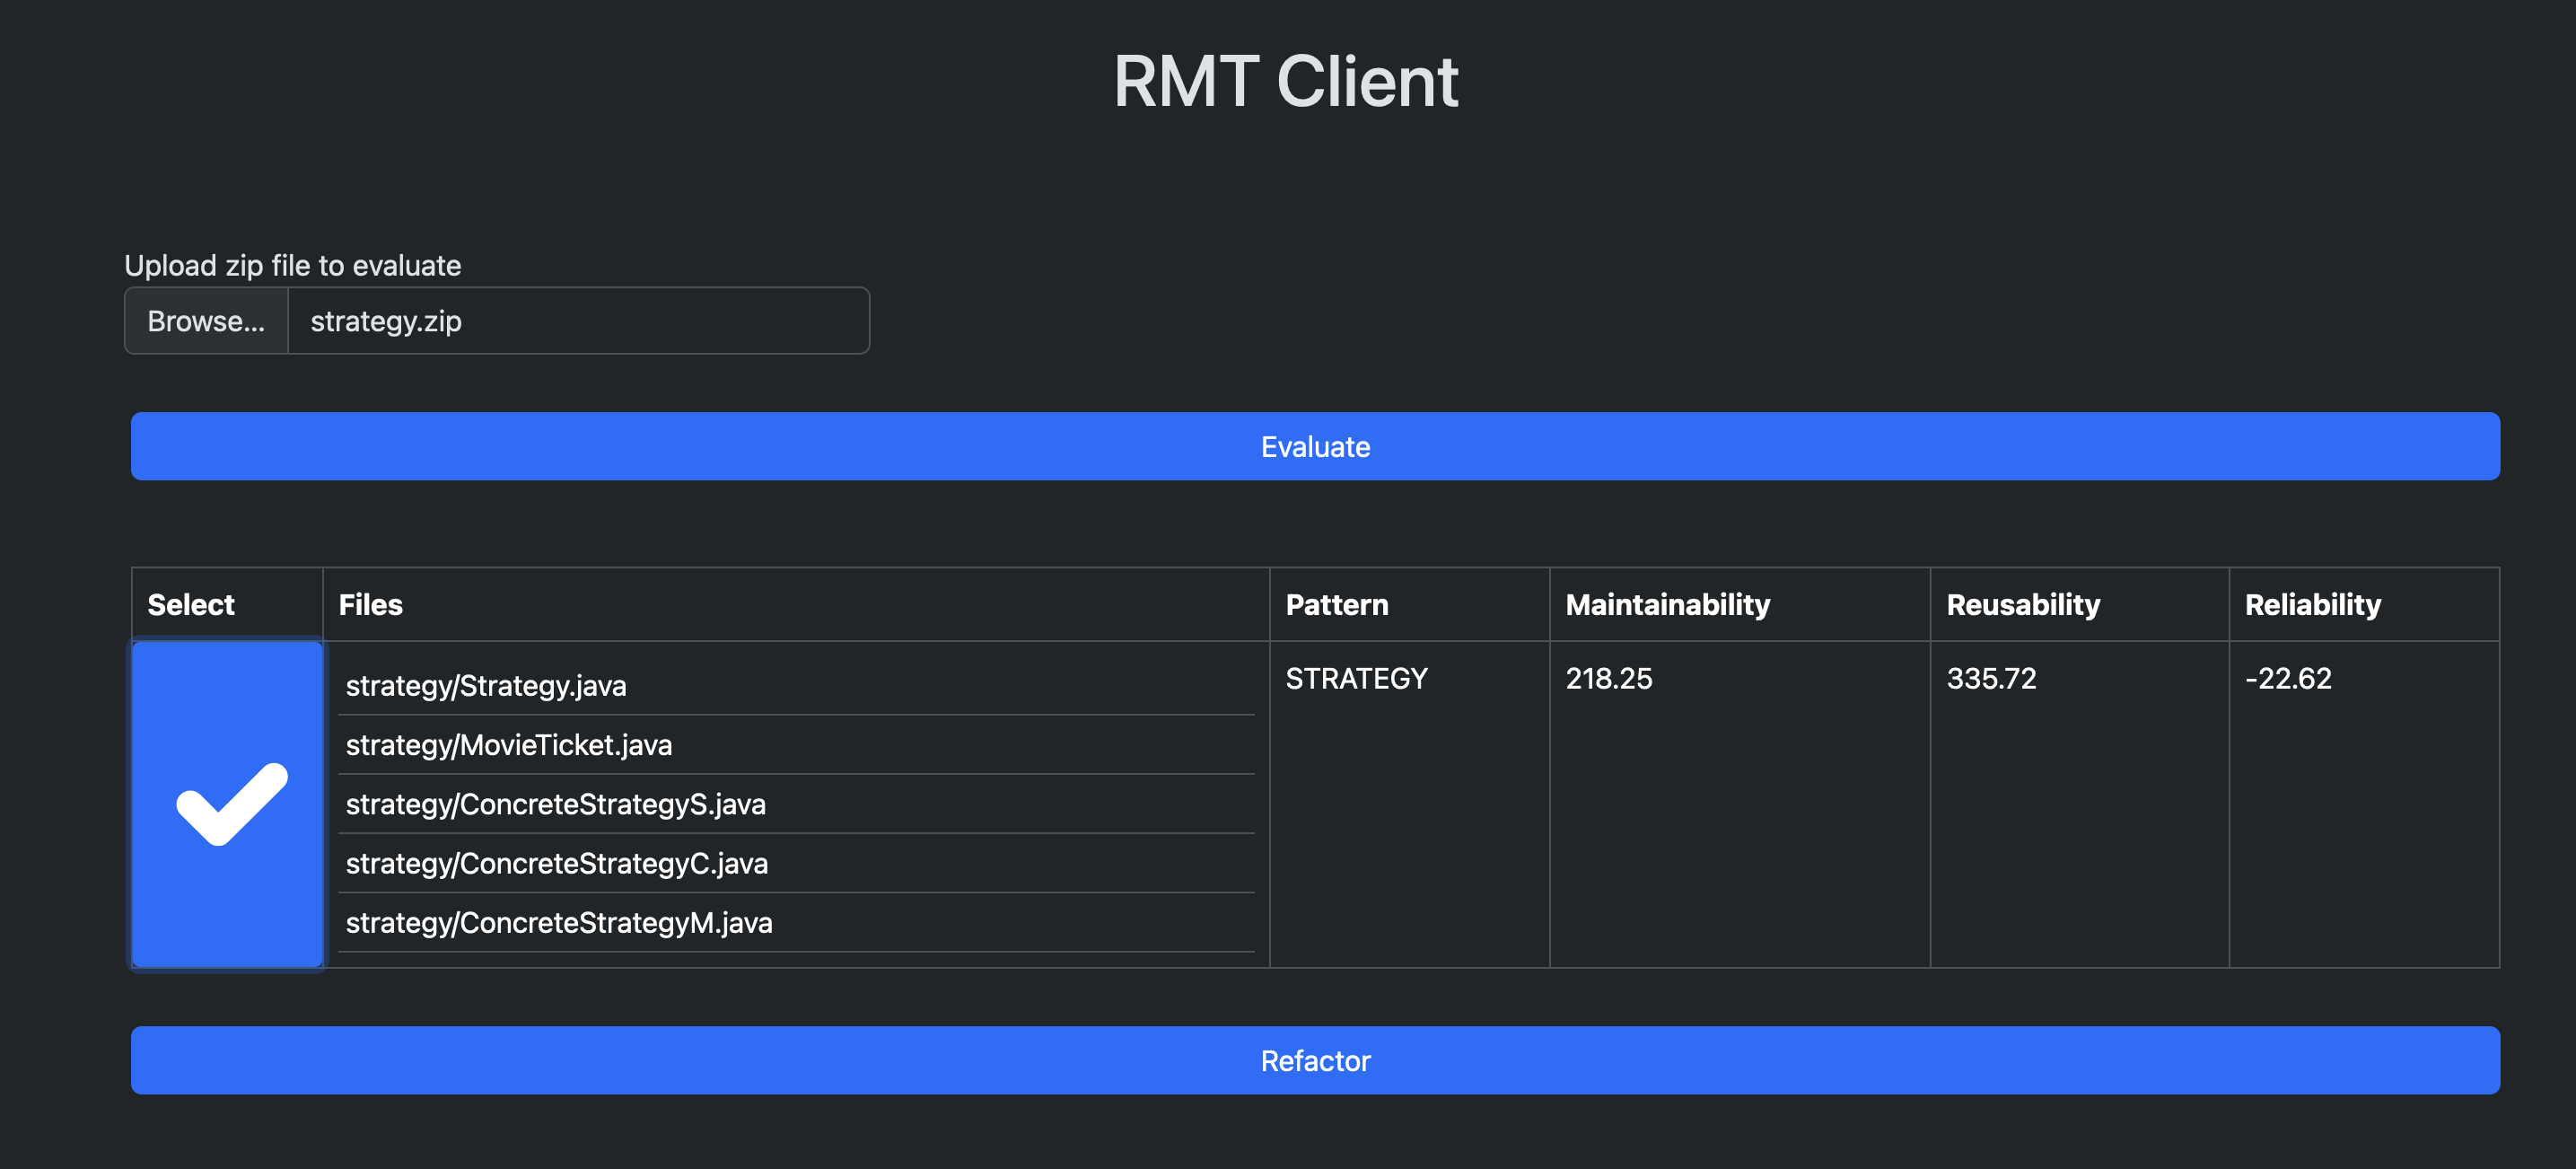
\includegraphics[width =\textwidth]{Chapter-5/Figures/rmt-strategy-client.png}
\SourceOrNote{Own authorship (2024)}
\end{figure}
\FloatBarrier

The \textcite{zafeiris2017automated} implements the template method using the jade-test-suit to exemplify the process. The \texttt{JICPPeer} class is the parent of the \texttt{JICPSPeer} class, which implements a method that has a \texttt{super} call; the refactoring extract code before and after the super call into new methods and replaces the super call to a method call with the same behavior. The maintainability, reusability, and reliability metrics are negative, showing a deterioration. It is represented in \Cref{fig-template-client}

\begin{figure}[ht!]
\caption{Refactored Project For Template Method}
\label{fig-template-client}
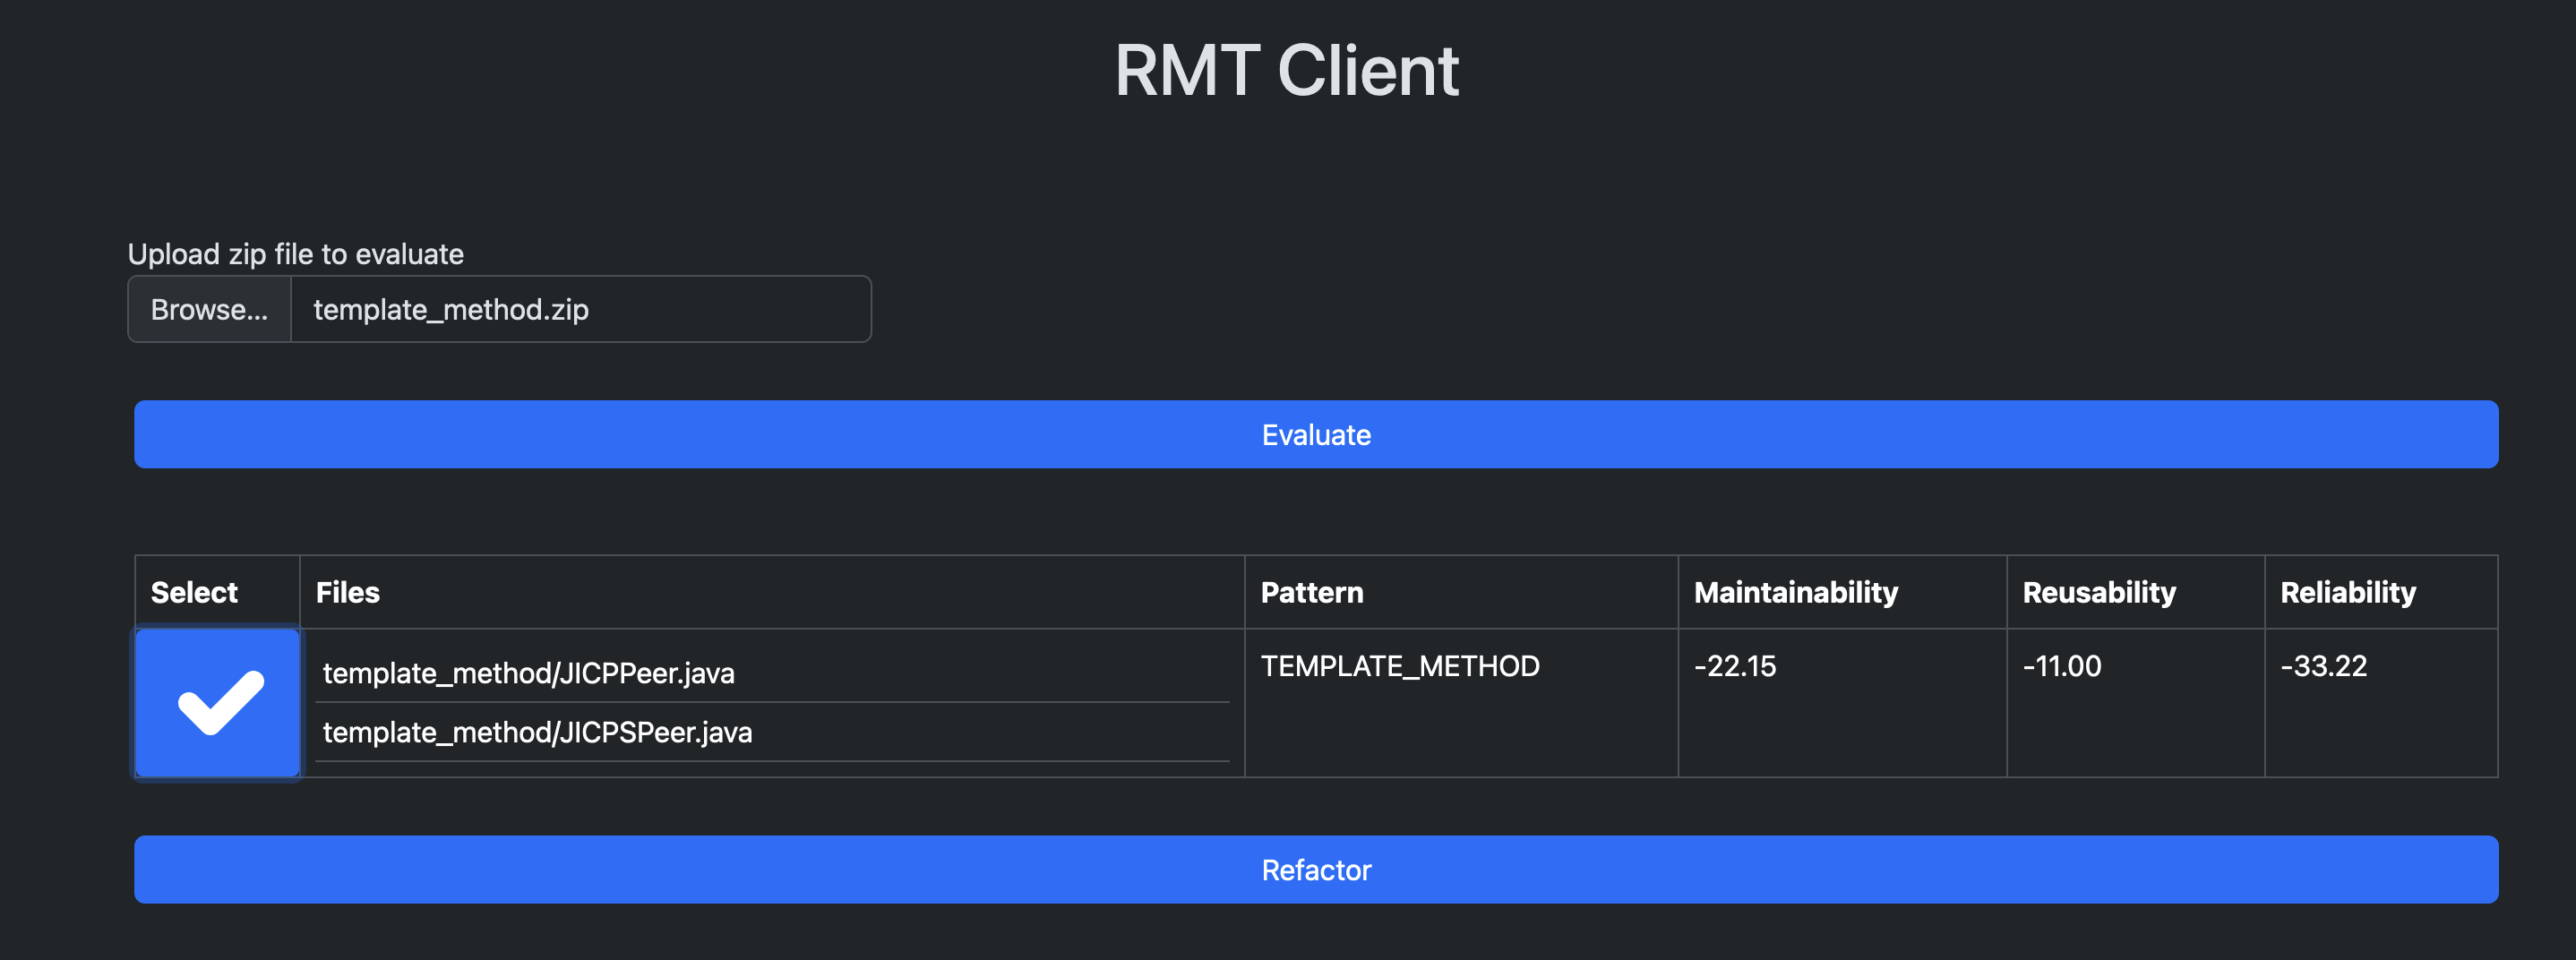
\includegraphics[width =\textwidth]{Chapter-5/Figures/rmt-template-client.png}
\SourceOrNote{Own authorship (2024)}
\end{figure}
\FloatBarrier

An additional approach to test the tool and ensure its quality will undergo a self-scanning procedure. The analysis was performed to test the effectiveness of the tool, with a focus on evaluating RMT and its next version, RMT 2.0. Examining both RMT versions showed that there were no elements that needed refactoring. 

\subsection{Testing With Real Projects}
\label{sub-testing-real}

The new version of the tool has to be tested against real-world projects to ensure that it does not break and maintains the initial functionality. To evaluate the RMT, \textcite{beluzzo2018abordagem}, select fifty projects from Github; from those projects, the RMT found candidate refactoring in seventeen projects. All these projects are shown on \cref{tab-projects-classes}; most of the projects have been updated after \cite{beluzzo2018abordagem} testing.

\begin{table}[!htbp]
  \centering
  \caption{List of Projects For Test Cases}
  \begin{tabular}{e{},{}@{}lc}
    \toprule
    \textbf{\#} & \textbf{Projects} & \textbf{Nº of classes} \\
    \midrule
    p1  & \href{https://github.com/evant/gradle-retrolambda.git}{https://github.com/evant/gradle-retrolambda.git}                               & 23  \\
    p2  & \href{https://github.com/Progether/JAdventure.git}{https://github.com/Progether/JAdventure.git}                                       & 64  \\
    p3  & \href{https://github.com/menacher/java-game-server.git}{https://github.com/menacher/java-game-server.git}                             & 187 \\
    p4  & \href{https://github.com/google/caliper.git}{https://github.com/google/caliper.git}                                                   & 269 \\
    p5  & \href{https://github.com/Devskiller/jfairy.git}{https://github.com/Devskiller/jfairy.git}                                             & 90  \\
    p6  & \href{https://github.com/jpush/jpush-api-java-client.git}{https://github.com/jpush/jpush-api-java-client.git}                         & 120 \\
    p7  & \href{https://github.com/dain/leveldb.git}{https://github.com/dain/leveldb.git}                                                       & 106 \\
    p8  & \href{https://github.com/census-instrumentation/opencensus-java.git}{https://github.com/census-instrumentation/opencensus-java.git}   & 626 \\
    p9  & \href{https://github.com/raml-org/raml-java-parser}{https://github.com/raml-org/raml-java-parser}                                     & 458 \\
    p10 & \href{https://github.com/Javacord/Javacord.git}{https://github.com/Javacord/Javacord.git}                                             & 1100 \\
    p11 & \href{https://github.com/maxmind/geoip-api-java.git}{https://github.com/maxmind/geoip-api-java.git}                                   & 28  \\
    p12 & \href{https://github.com/kwhat/jnativehook.git}{https://github.com/kwhat/jnativehook.git}                                             & 56  \\
    p13 & \href{https://github.com/cardillo/joinery.git}{https://github.com/cardillo/joinery.git}                                               & 51  \\
    p14 & \href{https://github.com/Kurento/kurento-java.git}{https://github.com/Kurento/kurento-java.git}                                       & 600 \\
    p15 & \href{https://github.com/joscha/play-authenticate.git}{https://github.com/joscha/play-authenticate.git}                               & 126 \\
    p16 & \href{https://github.com/caprica/vlcj.git}{https://github.com/caprica/vlcj.git}                                                       & 364 \\
    p17 & \href{https://github.com/careermonk/DataStructureAndAlgorithmsMadeEasyInJava.git}{https://github.com/careermonk/DataStructureAndAlgorithmsMadeEasyInJava.git} & 148 \\
    \bottomrule
  \end{tabular}
    \SourceOrNote{Own authorship (2024)}
  \label{tab-projects-classes}
\end{table}
\FloatBarrier

The tool was tested using the same updated projects. The \cref{tab-software-project-metrics} shows the results for the refactoring, with all the classes that could be refactored; the table displays the pattern by referring to the template method by T, the strategy by S, and the resulting metrics in percentage for each refactoring candidate.

Following a thorough analysis of the empirical results, it is immediately evident that the application of the factory method was not identified in any of the examined projects. The distribution of candidates for the template method and the strategy pattern is nearly balanced, with 14 classes favoring the strategy pattern characterizing 43.8\% of candidates and 18 classes corresponding to the template method equivalent to 56. 2\% of classes. Project two is not on the table as it had no candidates for refactoring.

Testing project two on RMT 1.0 shows a possible refactoring, but by debuting the tool and analyzing the post-refactoring files, was possible to find the same issue described in \cref{subsub-limitation}, where an Ast handler method has a bug that only returns one if statement from the method, making it accept the refactoring without evaluating the other ifs on the method.

Regarding the strategy method, it is plausible that specific projects may have two candidates for a single class. This occurrence is attributable to the candidate identification process, in which a class encompasses two methods suitable for refactoring. Analyzing the metrics, most projects demonstrated an improvement in maintainability and reusability, accompanied by a slight decrease in reliability. These findings suggest that strategy-based refactoring predominantly benefits developers based on the utilized metrics.

Nevertheless, the template method has shown marginal reductions in all metrics, with deviations that do not exceed a threshold of 1\%. The displayed metrics enable developers to make knowledgeable decisions about project refactoring; despite minor degradations in these metrics, a developer might still opt to refactor the class.

\begin{longtable}{ccp{5.1cm}ccc@{}}
%% Cabeçalho da primeira página
\caption{Refactored Projects Metrics and Classes}
\label{tab-software-project-metrics}                          \\[\belowcaptionskip]
\multicolumn{6}{@{}r@{}}{\textbf{(continue)}}                 \\[\belowcaptionskip]
\toprule%
\multicolumn{1}{@{}c}{\textbf{Project}}            &
\multicolumn{1}{c}{\textbf{Pattern}}               &
\multicolumn{1}{c}{\textbf{Class}}                 &
\multicolumn{1}{c}{\textbf{Maintainability}}       &
\multicolumn{1}{c}{\textbf{Reusability}}           &
\multicolumn{1}{c@{}}{\textbf{Reliability}}        \\
\midrule%
\endfirsthead%
%% Cabeçalho das páginas (exceto primeira e última)
\caption[]{Refactored Projects Metrics and Classes}           \\[\belowcaptionskip]
\multicolumn{6}{@{}r@{}}{\textbf{(continuation)}}             \\[\belowcaptionskip]
\toprule%
\multicolumn{1}{@{}c}{\textbf{Project}}            &
\multicolumn{1}{c}{\textbf{Pattern}}               &
\multicolumn{1}{c}{\textbf{Class}}                 &
\multicolumn{1}{c}{\textbf{Maintainability}}       &
\multicolumn{1}{c}{\textbf{Reusability}}           &
\multicolumn{1}{c@{}}{\textbf{Reliability}}        \\
\midrule%
\endhead%
%% Cabeçalho da última página
\caption[]{Refactored Projects Metrics and Classes}           \\[\belowcaptionskip]
\multicolumn{6}{@{}r@{}}{\textbf{(conclusion)}}               \\[\belowcaptionskip]
\toprule%
\multicolumn{1}{@{}c}{\textbf{Project}}            &
\multicolumn{1}{c}{\textbf{Pattern}}               &
\multicolumn{1}{c}{\textbf{Class}}                 &
\multicolumn{1}{c}{\textbf{Maintainability}}       &
\multicolumn{1}{c}{\textbf{Reusability}}           &
\multicolumn{1}{c@{}}{\textbf{Reliability}}        \\
\midrule%
\endlasthead%
%% Rodapé da última página
\bottomrule%
\LTSourceOrNote{Own authorship (2024)}           \\
\endlastfoot% 
  p1 & S & Feature.java & 3.25 & 5.45 & -0.90 \\
  p1 & S & Lib.java & 3.25 & 5.45 & -0.90 \\
  p3 & S & JetlangEventDispatcher.java & 0.24 & 0.38 & -0.06 \\
  p3 & T & AbstractNettyServer.java & -0.10 & -0.06 & -0.16 \\
  p3 & T & DefaultSessionEventHandler.java & -0.13 & -0.08 & -0.20 \\
  p4 & S & ShortDuration.java & 0.15 & 0.23 & 0 \\
  p5 & S & PlVATIdentificationNumberProvider.java & 0.43 & 0.71 & -0.16 \\
  p5 & T & FairyModule.java & -0.62 & -0.25 & -0.94 \\
  p6 & T & PlatformNotification.java & -0.20 & -0.10 & -0.30 \\
  p7 & S & Slices.java & 0.44 & 0.68 & -0.06 \\
  p7 & S & Slices.java & 0.44 & 0.68 & -0.06 \\
  p8 & S & BenchmarksUtil.java & 0.10 & 0.16 & -0.02 \\
  p8 & S & BenchmarksUtil.java & 0.10 & 0.16 & -0.02 \\
  p8 & S & StackdriverExportUtils.java & 0.07 & 0.10 & -0.02 \\
  p8 & T & AbstractMvcIntegrationTest.java & -0.03 & -0.02 & -0.04 \\
  p8 & T & HttpServletFilter.java & -0.03 & -0.02 & -0.05 \\
  p9 & T & ReferenceSuggester.java & -0.05 & -0.03 & -0.08 \\
  p10 & T & SlashCommandBuilderDelegateImpl.java & -0.02 & -0.02 & -0.04 \\
  p10 & T & TextableRegularServerChannelUpdater-DelegateImpl.java & -0.03 & -0.02 & -0.04 \\
  p10 & T & ServerThreadChannelUpdater-DelegateImpl.java & -0.04 & -0.02 & -0.06 \\
  p10 & T & ServerVoiceChannelUpdater-DelegateImpl.java & -0.03 & -0.02 & -0.05 \\
  p10 & T & ServerVoiceChannelUpdater-DelegateImpl.java & -0.05 & -0.03 & -0.08 \\
  p11 & S & LookupService.java & 3.21 & 4.82 & -0.03 \\
  p12 & T & NativeMouseEvent.java & -0.31 & -0.20 & -0.46 \\
  p12 & T & NativeInputEvent.java & -0.39 & -0.25 & -0.58 \\
  p13 & S & DataFrameAdapter.java & 0.43 & 0.69 & -0.08 \\
  p14 & S & JsonRpcConnectionListenerKurento.java & 0.05 & 0.08 & -0.02 \\
  p14 & T & AbstractJsonRpcClientWebSocket.java & -0.03 & -0.02 & -0.04 \\
  p15 & T & OAuth1AuthProvider.java & -0.18 & -0.10 & -0.28 \\
  p16 & T & TrackInfo.java & -0.12 & -0.09 & -0.18 \\
  p16 & T & Track.java & -0.18 & -0.13 & -0.26 \\
  p17 & S & FibonacciWithDP.java & 0.89 & 1.37 & -0.10 \\
  \bottomrule
\end{longtable}
\FloatBarrier

\section{Comparing RMT versions}
\label{sec-comparing}

Following the evaluation of the tool, the next stage involves assessing the efficacy of the RMT's remodeling. As noted in \cref{subsub-limitation}, the initial version of the tool demonstrated issues in handling 'if' statements within the Template Method and Strategy design patterns. Consequently, it impeded a direct comparison of metrics between the tools, as the refactoring results would inherently differ, leading to variations in the calculated results.

One of the hypotheses proposed through the refactoring of the tool is that RMT 2.0 exhibits superior performance compared to version 1.0. To validate this claim, both tools were subjected to a comparative analysis by executing the 16 projects of \cref{tab-projects-classes}. The experiments were carried out on a MacBook Air M1 with 8GB of RAM; all other programs were closed, and the computer was plugged in so it could deliver the most power.

For the first version, the MongoDB 5.0.28 \cite{mongo} database was deployed using Docker, complemented by the WildFly 19 \cite{wildfly} server for the service deployment. Adjustments were necessary to allocate JVM memory from 512 MB to 2048 MB on the wildfly server to successfully analyze larger projects.

In the second version, the entire deployment was containerized using Docker \cite{docker}. The database service was managed using Redis \cite{Redis} version 7.2.4, while Localstack \cite{localstack} version 3.02 was used to provision the SQS queue and S3 storage. The Spring Framework \cite{spring} incorporates an embedded server, eliminating the need for an external application server such as WildFly and enabling the application deployment as a container.

The \Cref{fig-time-chart} shows the execution times for the fifteen projects. In particular, project p8 failed to run under RMT 1.0, which caused an error on every attempt. The projects with a time difference greater than 50\% were tested three times to ensure that the computer did not cause the performance error at the time; the minimum time of the three executions is represented in the table. 

\begin{table}[!htbp]
    \label{tab-comparison-rmt}
    \centering
    \caption{Comparison of RMT 1.0 and RMT 2.0 Execution Time}
    \begin{tabular}{e{},{}@{}lllcc}
        \toprule
        \textbf{Projects} & \textbf{RMT 1.0} & \textbf{RMT 2.0} & \textbf{Diff In Seconds} & \textbf{Diff In Percentage} & \textbf{Project Size} \\
        \midrule
        p1 & 1,62768s & 0,72107s & 0,90661 & 55,70\% & 23 \\
        p3 & 14,75962s & 5,14317s & 9,61645 & 65,15\% & 187 \\
        p4 & 8,01335s & 3,15658s & 4,85677 & 60,61\% & 269 \\
        p5 & 9,76558s & 1,36931s & 8,39627 & 85,98\% & 90 \\
        p6 & 14,31251s & 1,6893s & 12,62321 & 88,20\% & 120 \\
        p7 & 3,27219s & 2,81377s & 0,45842 & 14,01\% & 106 \\
        p9 & 22,59097s & 3,4106s & 19,18037 & 84,90\% & 458 \\
        p10 & 141,6649s & 24,86174s & 116,80316 & 82,45\% & 1100 \\
        p11 & 3,4375s & 1,3395s & 2,098 & 61,03\% & 28 \\
        p12 & 3,29823s & 1,29021s & 2,00802 & 60,88\% & 56 \\
        p13 & 2,26107s & 1,77315s & 0,48792 & 21,58\% & 51 \\
        p14 & 37,42521s & 7,69026s & 29,73495 & 79,45\% & 600 \\
        p15 & 7,33497s & 1,14457s & 6,1904 & 84,40\% & 126 \\
        p16 & 14,69265s & 3,81467s & 10,87798 & 74,04\% & 364 \\
        p17 & 2,09381s & 1,33635s & 0,75746 & 36,18\% & 148 \\
        \bottomrule
    \end{tabular}
    \SourceOrNote{Own authorship (2024)}
\end{table}
\FloatBarrier

Through detailed analysis of execution durations, it became apparent that the projects exhibiting extended execution times comprised more classes as in \Cref{fig-time-by-size} and were refactored for the template method. Specifically, projects p3, p5, p6, p9, p10, p12, p14, p15, and p16, which incorporated the Template Method refactoring, demonstrated a significant discrepancy in execution time when contrasting both tool versions. This discrepancy arises due to performance-focused optimizations implemented within the method code and the overall tool.

\begin{figure}[ht!]
\caption{Execution time difference between RMT version}
\label{fig-time-chart}
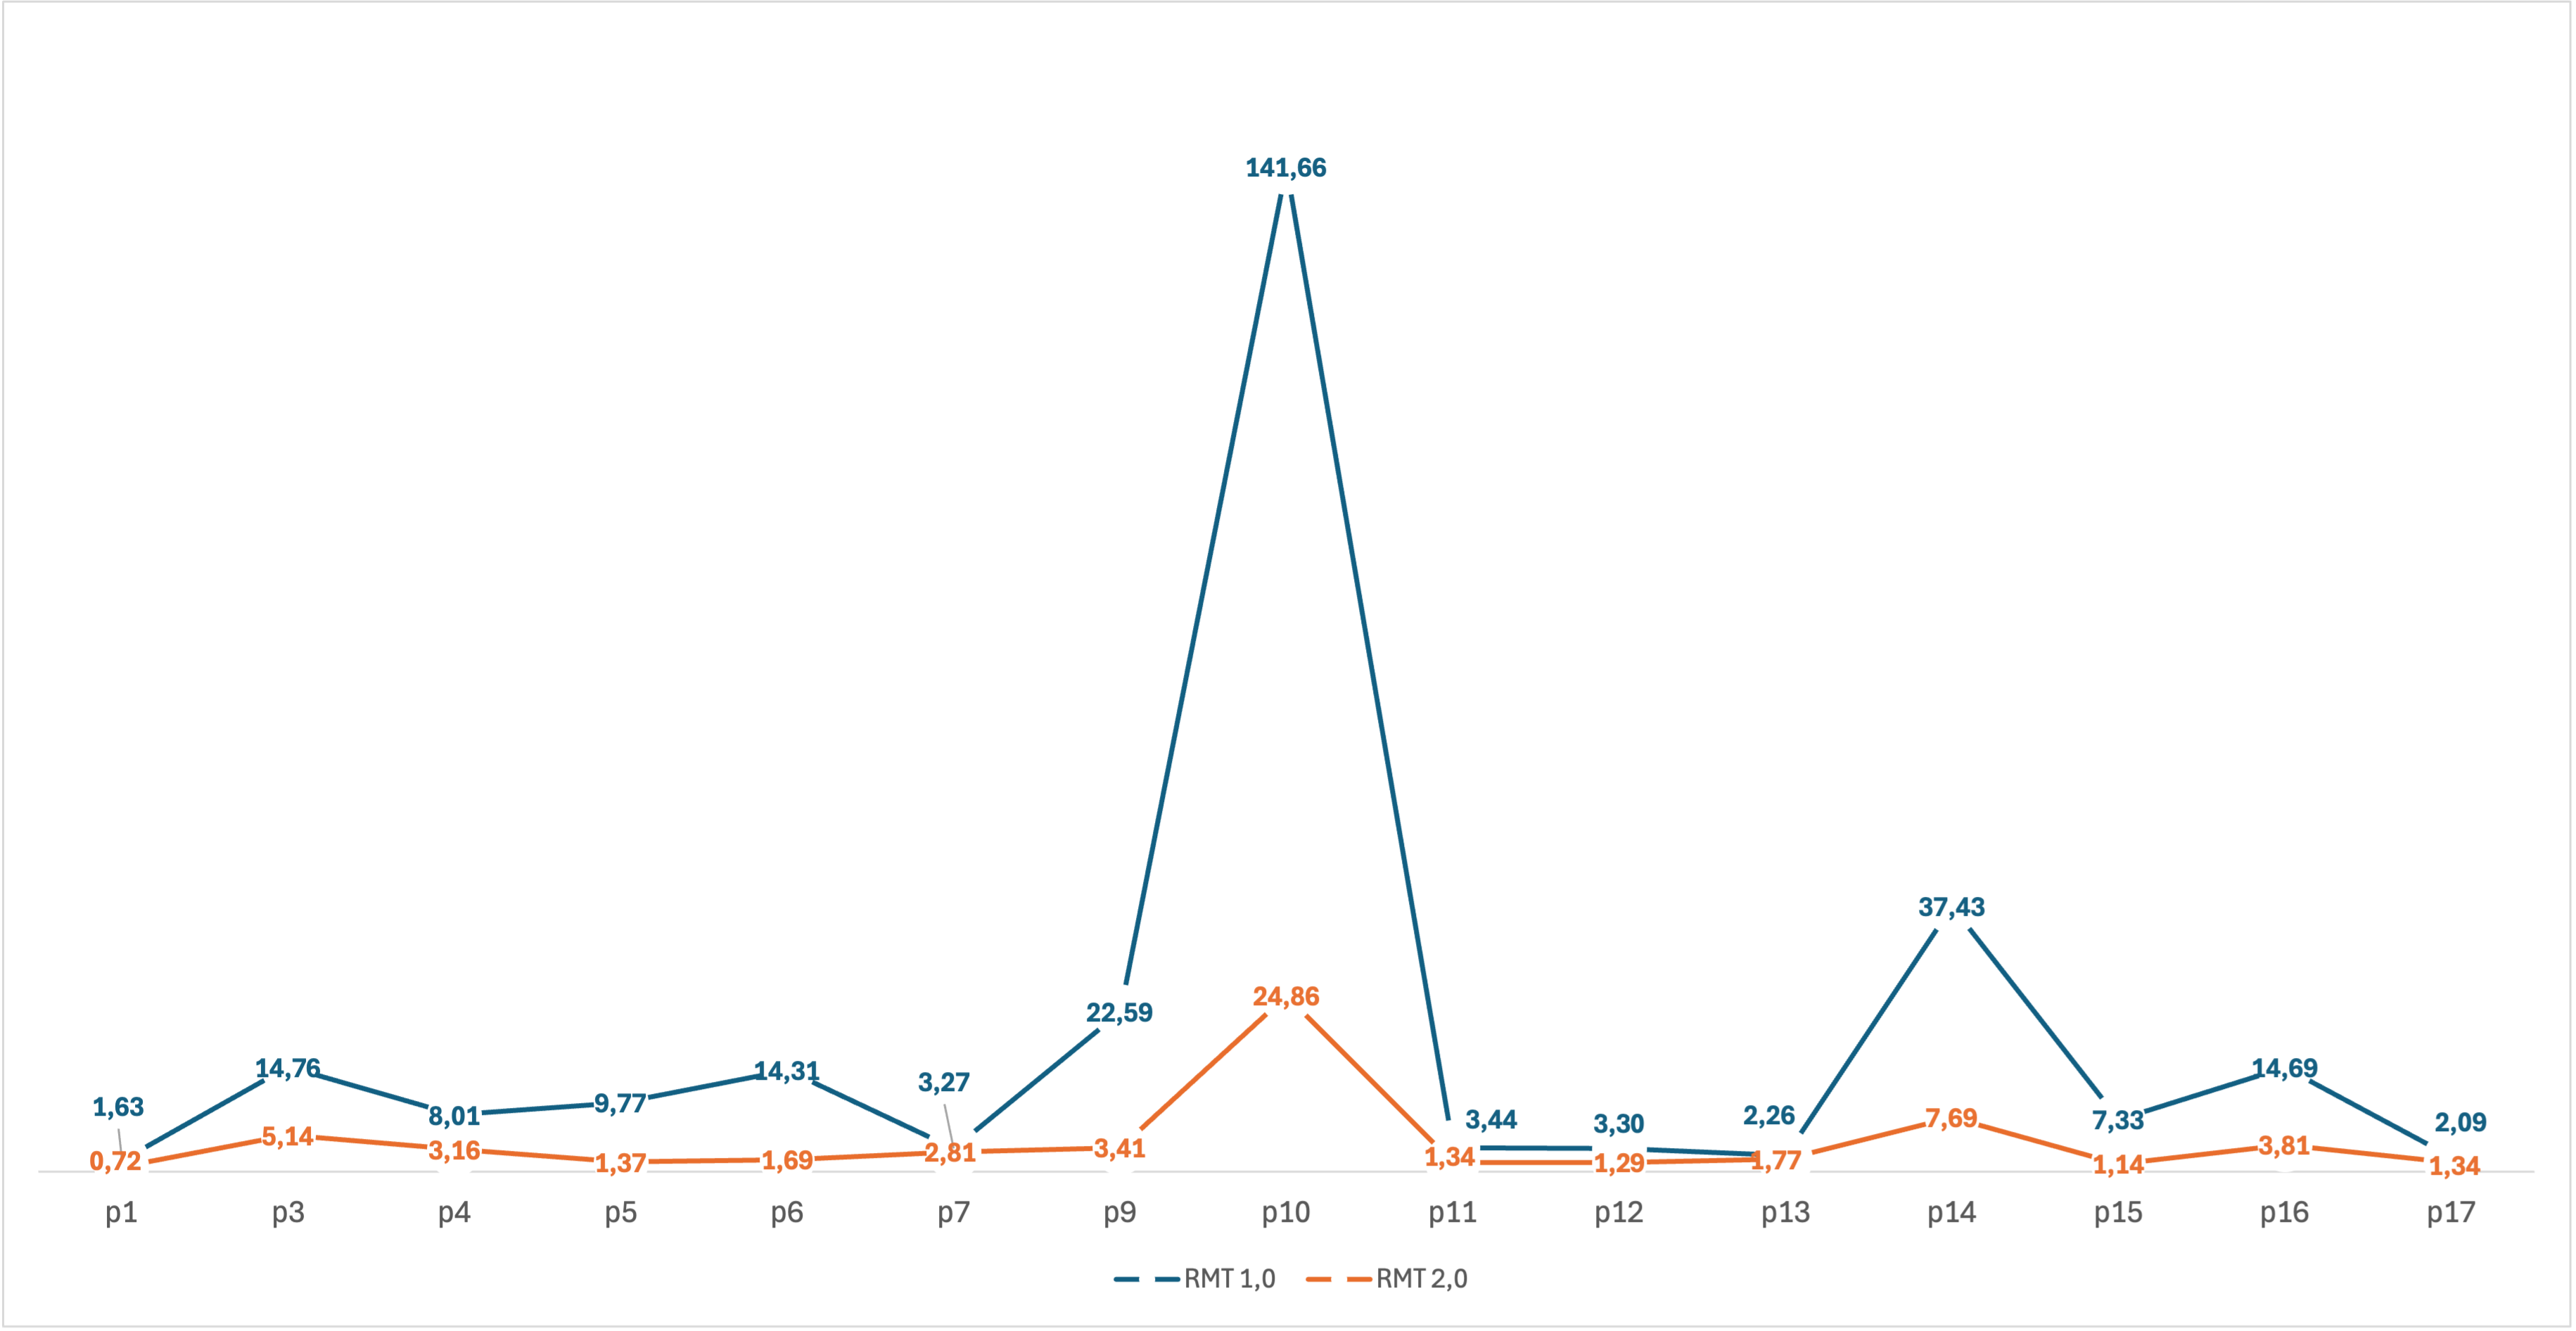
\includegraphics[width =\textwidth]{Chapter-5/Figures/time-diff.png}
\SourceOrNote{Own authorship (2024)}
\end{figure}
\FloatBarrier

The RMT 2.0 exhibited a substantial decrease in execution time by 63.64\%. This reduction was particularly pronounced in projects p5, p6, p9, p10, p14, p15, and p16, with over 80\% reductions recorded in projects p5, p6, p9, p10, and p15. In particular, excluding p5, all these projects have more than 100 classes. The larger difference between projects is in p9 and p10, which have 458 and 1100 classes, respectively. 

\begin{figure}[ht!]
\caption{Execution time difference by project size between RMT version}
\label{fig-time-by-size}
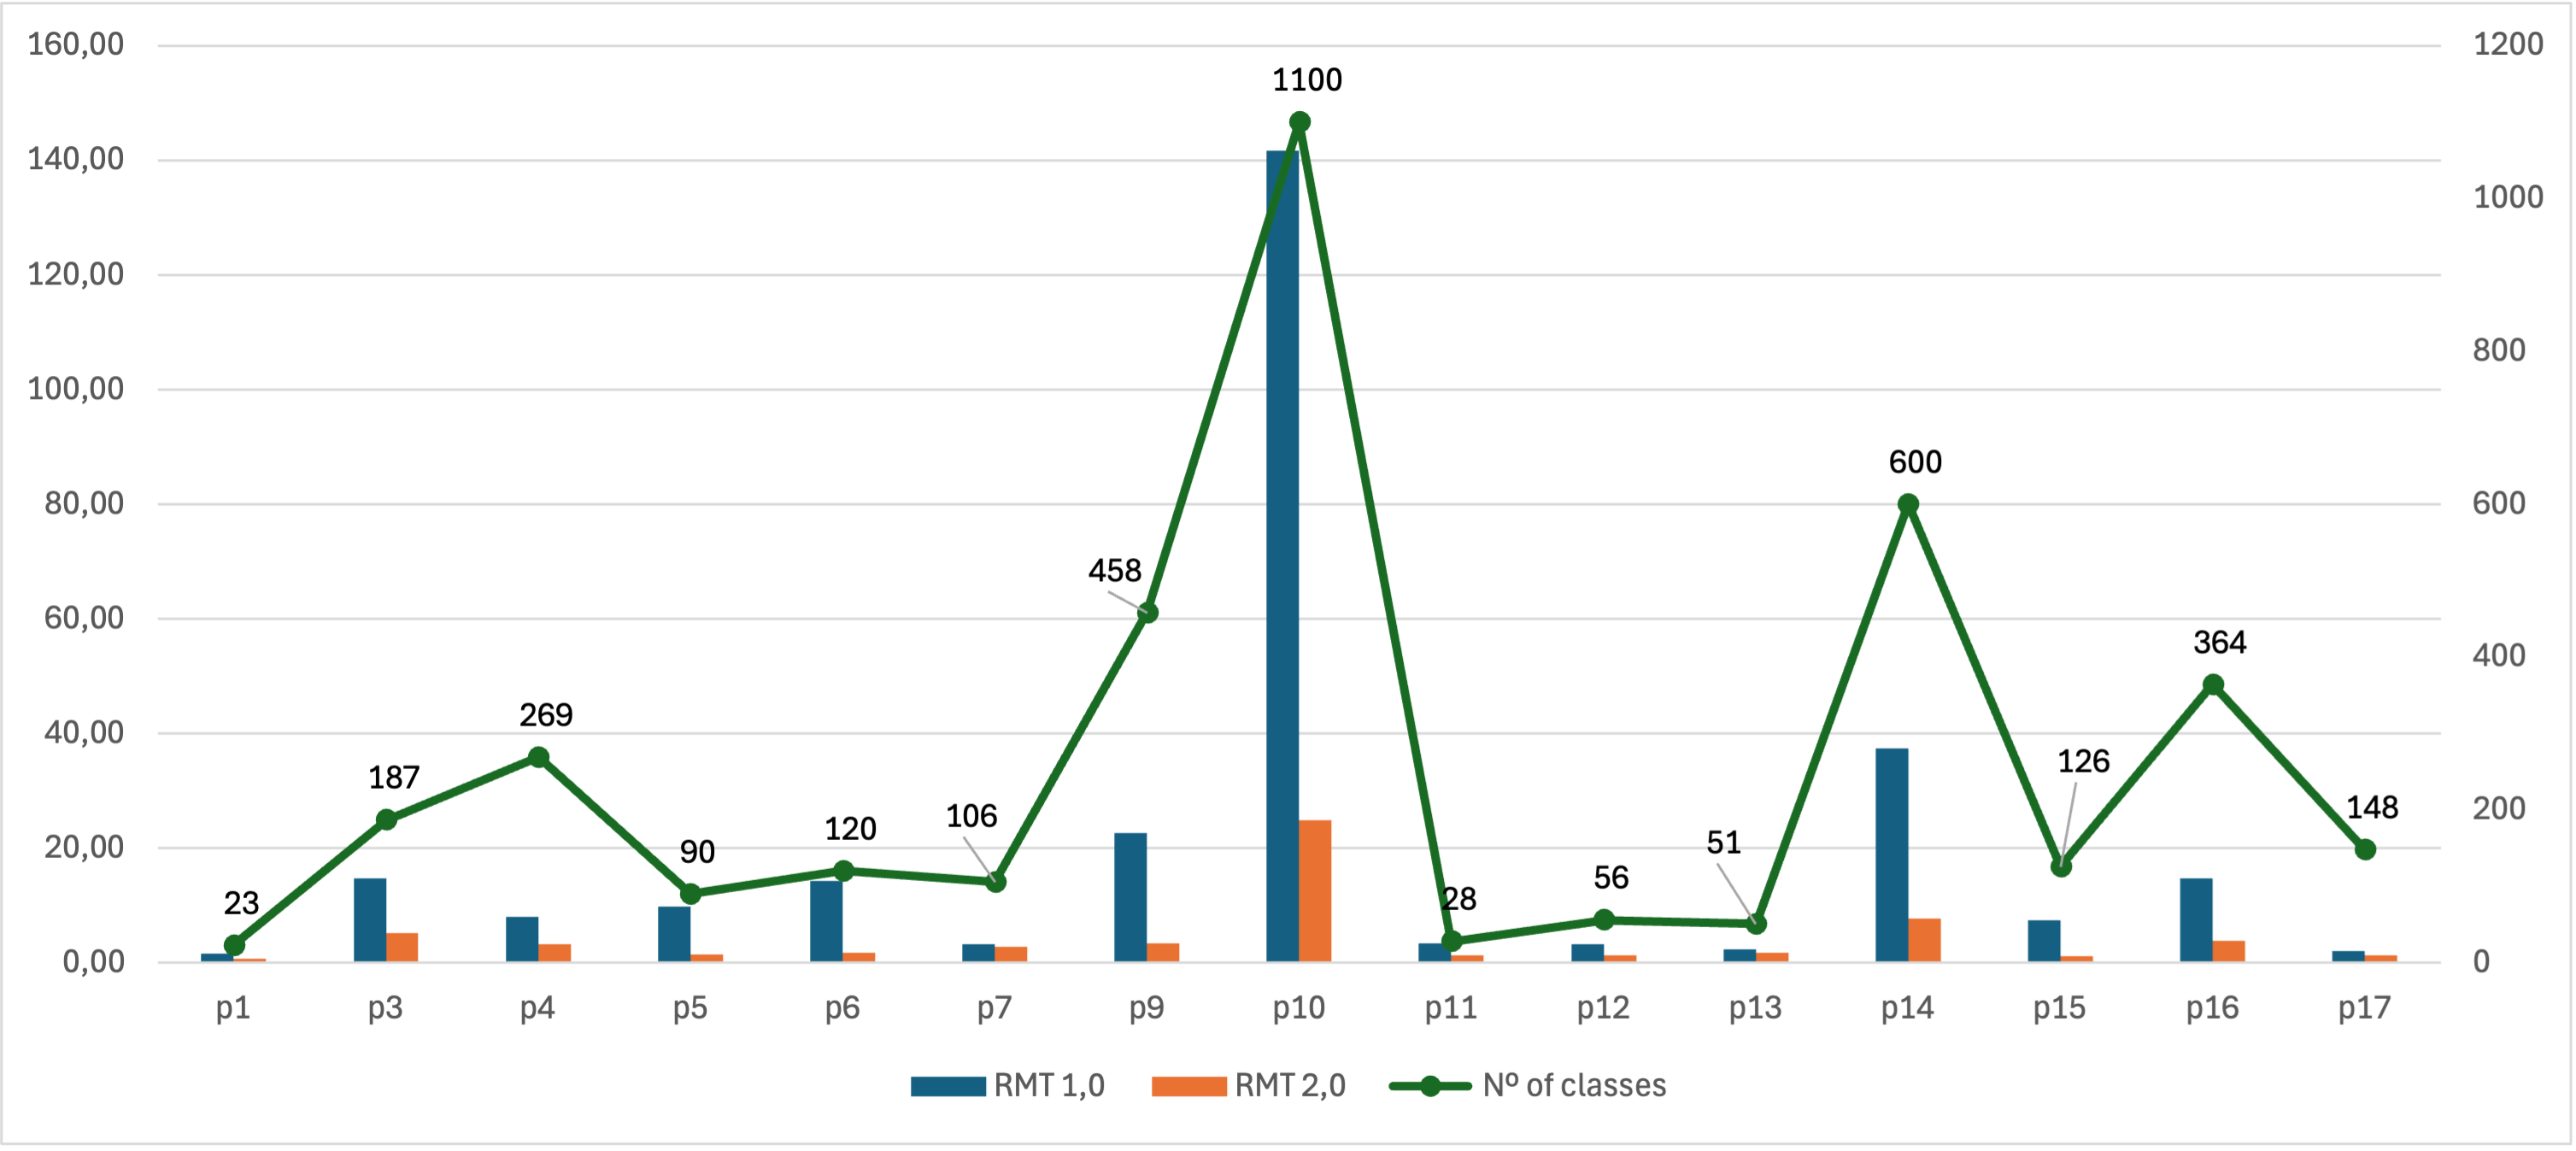
\includegraphics[width =\textwidth]{Chapter-5/Figures/time-per-project-size.png}
\SourceOrNote{Own authorship (2024)}
\end{figure}
\FloatBarrier

The projects p1, p4, p7, p13, p14, and p17 were exclusively refactored using the strategy pattern. These projects exhibit the shortest overall execution time and the smallest variance in execution duration, indicating that the strategy refactoring approach is more optimized for both tool versions. 

\section{Closing Remarks}
\label{sec-closing-results}

Upon comprehensive analysis of the datasets from both projects, it has been concluded that the proposal for enhancing the tool has been successful, yielding a temporal efficiency improvement of 63.64\%. The tool's implementation has been streamlined, necessitating containerization solutions such as Docker or Podman for execution. An automated script has been developed to compile and execute the project, concurrently deploying all requisite infrastructure within Docker.